\documentclass[12pt,letterpaper]{article}

\usepackage[hmargin=1in,bottom=1in,top=1in]{geometry}
\usepackage[latin1]{inputenc}
\usepackage{amsmath}
\usepackage{amsfonts}
\usepackage{amssymb}
\usepackage{graphicx}
\usepackage{url}
\usepackage[toc,page]{appendix}
\usepackage{setspace}
\usepackage{pdfpages}
\usepackage{mdwlist}

\usepackage{ulem}
\normalem

% push footnotes to the bottom of the page unconditionally
\usepackage[bottom]{footmisc}

\bibliographystyle{IEEEtran}

\setlength{\parindent}{0in}
\setlength{\parskip}{1.0 \baselineskip}
\setlength{\footnotesep}{1.0 \baselineskip}
\setlength{\skip\footins}{2.0 \baselineskip}

\newenvironment{enumeration}{
	\setlength{\topsep}{0.0pt}
	\setlength{\partopsep}{0pt}
	\setlength{\parskip}{0pt}
	\setlength{\parsep}{0pt}
	\begin{enumerate}
		\setlength{\itemsep}{0pt}}
	{\end{enumerate}}

\newenvironment{itemlist}{
	\setlength{\topsep}{0pt}
	\setlength{\partopsep}{0pt}
	\setlength{\parskip}{0pt}
	\setlength{\parsep}{0pt}
	\begin{itemize}
		\setlength{\itemsep}{0pt}}
	{\end{itemize}}

\newcommand{\sectref}[1]{Section \ref{#1}}
\newcommand{\figref}[1]{Figure \ref{#1}}
\newcommand{\tableref}[1]{Table \ref{#1}}

\usepackage{enumitem}
\setlist{nolistsep}

\begin{document}

\begin{titlepage}
\begin{center}


\includegraphics[scale=1.0]{ecelogo.png}

\vspace{1 \baselineskip}

\textsc{
\Large University of Toronto\\
\large Department of Electrical and Computer Engineering \\
\large ECE496 Design Project
}

\vspace{2 \baselineskip}

{\Large \bfseries Virtual FPGA fabrics} \\
{\Large \bfseries Implementation of a Virtual FPGA Architecture}

\vspace{2 \baselineskip}

{\large \bfseries Individual Progress Report} \\
%{\large \bfseries Final Version}

\vspace{2 \baselineskip}

{\large January 17, 2012}

\vfill

\begin{tabular*}{4in}{l @{\extracolsep{\fill}} l}
\textbf{Neil Isaac} & \texttt{n.isaac@utoronto.ca} \\ & \\
\emph{Project ID:} & 2011017 \\
\emph{Supervisor:} & Jason Anderson \\
\emph{Administrator:} & Ross Gillett \\
\emph{Section:} & \#7 \\
\end{tabular*}

\end{center}
\end{titlepage}

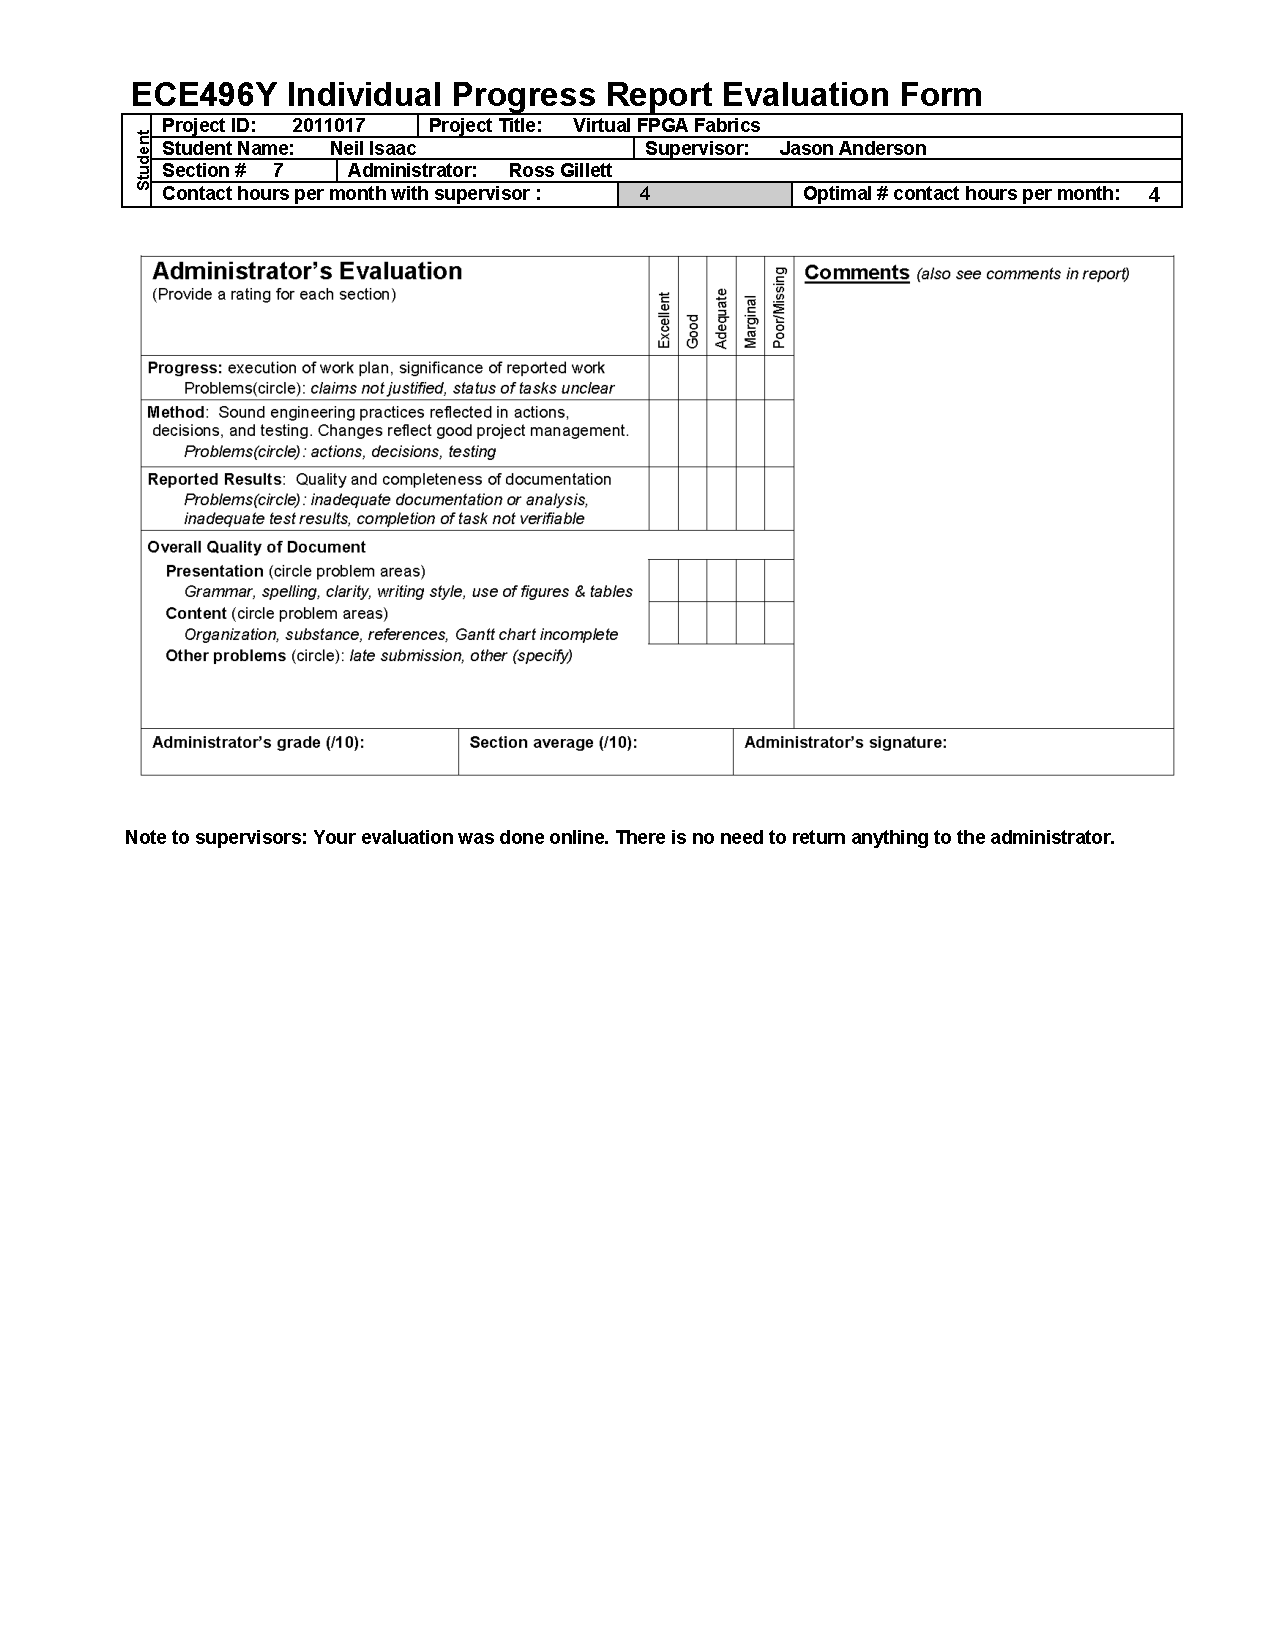
\includepdf{cover-sheet-neil.pdf}

\onehalfspace

\thispagestyle{empty}
\section*{Executive Summary}

Our project is progressing well and we are optimistic that we can meet our deadlines.
We initially planned optimistic deadline for long-term tasks, but left a couple of months of slack at the end of the project.
Now that we have begun those tasks, we have adjusted the gantt chart to reflect more realistic expectations for some of those tasks.
The slack time is now reflected within the time allocations for the tasks themselves.

My main contributions to the project are:
\begin{itemize}
\item components of the Virtual FPGA verilog design,
\item the third-partly tool flow to produce placement and routing data,
\item software to convert the placement and routing into a programmable bitstream, and
\item I will work on improving the quality of this software and support future improvements to the verilog design.
\end{itemize}

We have completed the basic components of the design, and the components all work individually, but need to do extensive debugging work to get it all working together.
Once we complete this debugging, we have a number of improvements planned to improve the quality of the virtual FPGA (in terms of usability to researchers, as well as its efficiency.)
These improvements are not necessary for a proof-of-concept, or for a fully functional demo.

We are confident that we can complete these remaining tasks before the design fair.




\pagebreak
\pagenumbering{arabic}




\section{Individual Progress and Contributions}

This section lists the four major tasks I have been responsible for.
The respective tasks are discussed in more detail in section 2, with emphasis on my own contributions.
The complete gantt chart, showing all of our group's tasks is included in Appendix A.

\begin{tabular}{|l|l|l|l|l|l|l|}
\hline
\textbf{Task title} & \textbf{Category} & \textbf{Status} & \textbf{Original date} & \textbf{New date} \\ \hline
\hline
1. Virtual FPGA Verilog code & hardware & debugging & Aug-Dec 15 & Aug-Jan 15 \\ \hline
2. External tool flow & tools & completed & Dec 1-Dec 15 & Dec 1-Dec 15 \\ \hline
3. Bitstream generation software & software & debugging & Dec 1-Dec 15 & Dec 1-Feb 15 \\ \hline
4. Stress-testing and improvement & testing & not started & Dec 15-Apr 1 & Jan 15-Apr 1 \\ \hline
\end{tabular}




\section{Information on Individual Milestones}

\begin{tabular}{|p{6.4in}|}
\hline
\textbf{1. Virtual FPGA Verilog code} \\
\emph{Category:} hardware \\
\emph{Original date:} August - December 15 \\
\emph{New date:} August - January 15 \\
\hline
\textbf{Responsibility:} Neil, Keyi \\
The components I wrote were the UART, logic block, connection block, and tile grid. \\
% Keyi: logic element, logic block, shift multiplexing, switch block, logic tile, grid boundary, tile optimization
\hline
\textbf{Status:} debugging; future improvements are planned \\
\vspace{-1em}
\begin{itemize}
\item Verilog code for basic virtual FPGA is complete.
\item Debugging work is required to get it to work in new configuration.
\item Future improvements will aim to to reduce the size of the circuit.
\end{itemize} 
\vspace{-1em} \\
\hline
\textbf{Actions} \\
\vspace{-1em}
\begin{itemize}
\item I wrote the UART, logic block, and connection block modules.
\item I worked on integrating them into the tile grid of the virtual FPGA design.
\item Serial data transmission over the UART seems is prone to data corruption with some of the hardware we have.
\end{itemize} 
\vspace{-1em} \\
\hline
\textbf{Decisions} \\
\vspace{-1em}
\begin{itemize}
\item The connectivity architecture of our modules was decided by taking the simplest approach supported by the placement and routing tool \emph{VPR}.
\item We implemented all the memory elements of the virtual FPGA circuit (including routing switches and logic tables) using native logic elements on the Virtex 5 board, configured as shift registers, as we described in the proposal document.
\item To address the UART corruption issues, I added a parity bit to each byte sent to program the virtual FPGA in the bitstream. If a parity bit doesn't match the byte, it can try to resend the byte. This was not good enough for large bitstreams, because sometimes 2 bits with flip within the byte, so the parity bit will still be `correct', but the byte isn't valid. To address this, I changed the hardware to send every byte received by the board back to the computer to verify it. If bytes are returned and are incorrect, it can't recover, but the user can try sending the bitstream again. If this remains a serious issue, I can adapt the programming protocol to allow it to replace the previous byte if it doesn't match when it is sent back to the computer.
\end{itemize} 
\vspace{-1em} \\
\hline
\textbf{Testing, verification and results} \\
\vspace{-1em}
\begin{itemize}
\item To test the virtual FPGA at this stage, we created the bitstream (programming) files manually to implement small test circuits. Functionality was tested using switches and LEDs.
\end{itemize} 
\vspace{-1em} \\
\hline
\end{tabular}




\begin{tabular}{|p{6.4in}|}
\hline
\textbf{2. External tool flow} \\
\emph{Category:} tools \\
\emph{Original date:} December 1 - December 15 \\
\emph{New date:} December 1 - December 15 \\
\hline
\textbf{Responsibility:} Neil \\
\hline
\textbf{Status:} completed \\
Third-party tools will be used to produce the placement and routing for our input circuits.
These tools are: \emph{odin} (synthesis), \emph{abc} (technology mapping), \emph{t-vpack} (clustering) and \emph{VPR} (placement and routing). \\
\hline
\textbf{Actions} \\
\vspace{-1em}
\begin{itemize}
\item Wrote a test circuit, shown in Appendix B.
\item Verified that the tools will run using each others' outputs.
\item A bug in \emph{abc} results in it deleting clock information in circuit descriptions.
\end{itemize} 
\vspace{-1em} \\
\hline
\textbf{Decisions} \\
The bug in \emph{abc} can be worked around, subject to several limitations.
For the time being, I avoided it by writing an \emph{awk} script to process the output from \emph{abc} to add the clock information back in.
Implicitly in this script, I assume that there is only one clock in the design, and it is always called ``clk'', which are both limiting assumptions.
Ideally in the future, we will find a patched version of \emph{abc}, or will write more complex software to read the input file and interpolate less limited clock information.
The temporary \emph{awk} script is shown below:
\begin{verbatim}{    if ($1 == ".latch") { print $1, $2, $3, "re", "top^clk", $4; }
     else { print $0; }    }\end{verbatim}
\\ \hline
\textbf{Testing, verification and results} \\
\vspace{-1em}
\begin{itemize}
\item Checked the 4 output files manually for correctness and to verify that they provide adequate information to reproduce the circuit's function, placement, and routing on our virtual FPGA.
\item A screenshot of \emph{VPR} showing the placement and routing is shown in Appendix C.
\end{itemize} 
\vspace{-1em} \\
\hline
\end{tabular}




\begin{tabular}{|p{6.4in}|}
\hline
\textbf{3. Bitstream generation software} \\
\emph{Category:} software \\
\emph{Original date:} December 1- December 15 \\
\emph{New date:} December 1 - February 15 \\
\hline
\textbf{Responsibility:} Neil \\
\hline
\textbf{Status:} debugging \\
\vspace{-1em}
\begin{itemize}
\item Code is feature-complete for prototype design.
\item Working Verilog FPGA circuit is required to verify correctness.
\item Changes will be required to reflect future changes to hardware design.
\end{itemize} 
\vspace{-1em} \\
\hline
\textbf{Actions} \\
\vspace{-1em}
\begin{itemize}
\item The four inputs required to generate the bitstream are: the logic functions (in BLIF format) from \emph{odin} and \emph{abc}, the netlist from \emph{t-vpack}, and the placement and routing files from \emph{VPR}.
\item All of the information needed is in these files, but it needs to be inferred by cross-referencing between the files. This was more complicated than expected, so it took longer then initially planned.
\item Once I built a software model containing the data required, I wrote functions to loop over it and generate the bit patterns that will ultimately be programmed.
\item Once all the bit patterns are ready, they are combined into bytes before being programmed to the virtual FPGA over a serial connection.
\end{itemize} 
\vspace{-1em} \\
\hline
\textbf{Decisions} \\
\vspace{-1em}
\begin{itemize}
\item I wrote this software in Python 2.x because it is not performance critical, and the high-level abstractions available in Python speed up the development process.
\item One technical issue that came up is that some of the bit patterns are not evenly divisible into 8-bit bytes, so all of the patterns have to be compiled before they can be packed into bytes. For example, the patterns \texttt{100110} and \texttt{1100001101} should be combined into the bytes \texttt{10011011 00001101}, not \texttt{00100110 00000011 00001101} (by padding each individual pattern.)
\item Since the bitstream is programmed serially, the first hardware in the programming chain corresponds to the last bits in the bitstream.  This means that the bitstream is in reverse order of the intuitive numerical indices of the hardware.  This has led to a lot of trivial mistakes in the programming that I fixed gradually.
\end{itemize} 
\vspace{-1em} \\
\hline
\textbf{Testing, verification and results} \\
\vspace{-1em}
\begin{itemize}
\item I am testing basic functionality using the simple circuit in Appendix B.
\item This program outputs a text file containing each pattern in the bitstream which I can examine by hand, so I can test the software without the virtual FPGA circuit.
\item Extensive testing is covered by task \#4.
\end{itemize} 
\vspace{-1em} \\
\hline
\end{tabular}




\begin{tabular}{|p{6.4in}|}
\hline
\textbf{4. Stress-testing and improvement} \\
\emph{Category:} testing, hardware \\
\emph{Original date:} December 15 - April \\
\emph{New date:} January 15 - April \\
\hline
\textbf{Responsibility:} Neil, Keyi \\
I will focus on verification and improvements in the tool flow and bitstream software. \\
\hline
\textbf{Status:} not started \\
We will begin extensive verification and improvement once the prototype works. \\
\hline
\textbf{Actions} n/a \\
\hline
\textbf{Decisions} n/a \\
\hline
\textbf{Testing, verification and results} \\
\vspace{-1em}
\begin{itemize}
\item Make sure clocked logic works properly.
\item Make sure signal routing is always correct.
\item Make sure designs with hierarchical modules can be compiled.
\item Develop a way for the user to assign their inputs and outputs to specific pads (the peripheral input/output blocks) on the virtual FPGA.
\end{itemize} 
\vspace{-1em} \\
\hline
\end{tabular}





\section{Progress Assessment}

Our project is progressing well and we are optimistic that we can meet our deadlines.
Note that we initially planned optimistic deadline for long-term tasks, but left a couple of months of slack at the end of the project.
Now that we have begun those tasks, we have adjusted the gantt chart to reflect more realistic expectations for some of those tasks.
The slack time is now reflected within the time allocations for the tasks themselves.

We have completed the basic components of the design, and the components all work individually, but need to do extensive debugging work to get it all working together.
Once we complete this debugging, we have a number of improvements planned to improve the quality of the virtual FPGA (in terms of usability to researchers, as well as its efficiency.)
These improvements are not necessary for a proof-of-concept, or for a fully functional demo.

We are confident that we can complete these remaining tasks before the design fair.



%\pagebreak
%\nocite{*} % show uncited entries in the bibliography
%\bibliography{ref}
%\addcontentsline{toc}{section}{References}



\pagebreak
\begin{appendices}



\pagebreak

\section{Gantt Chart}
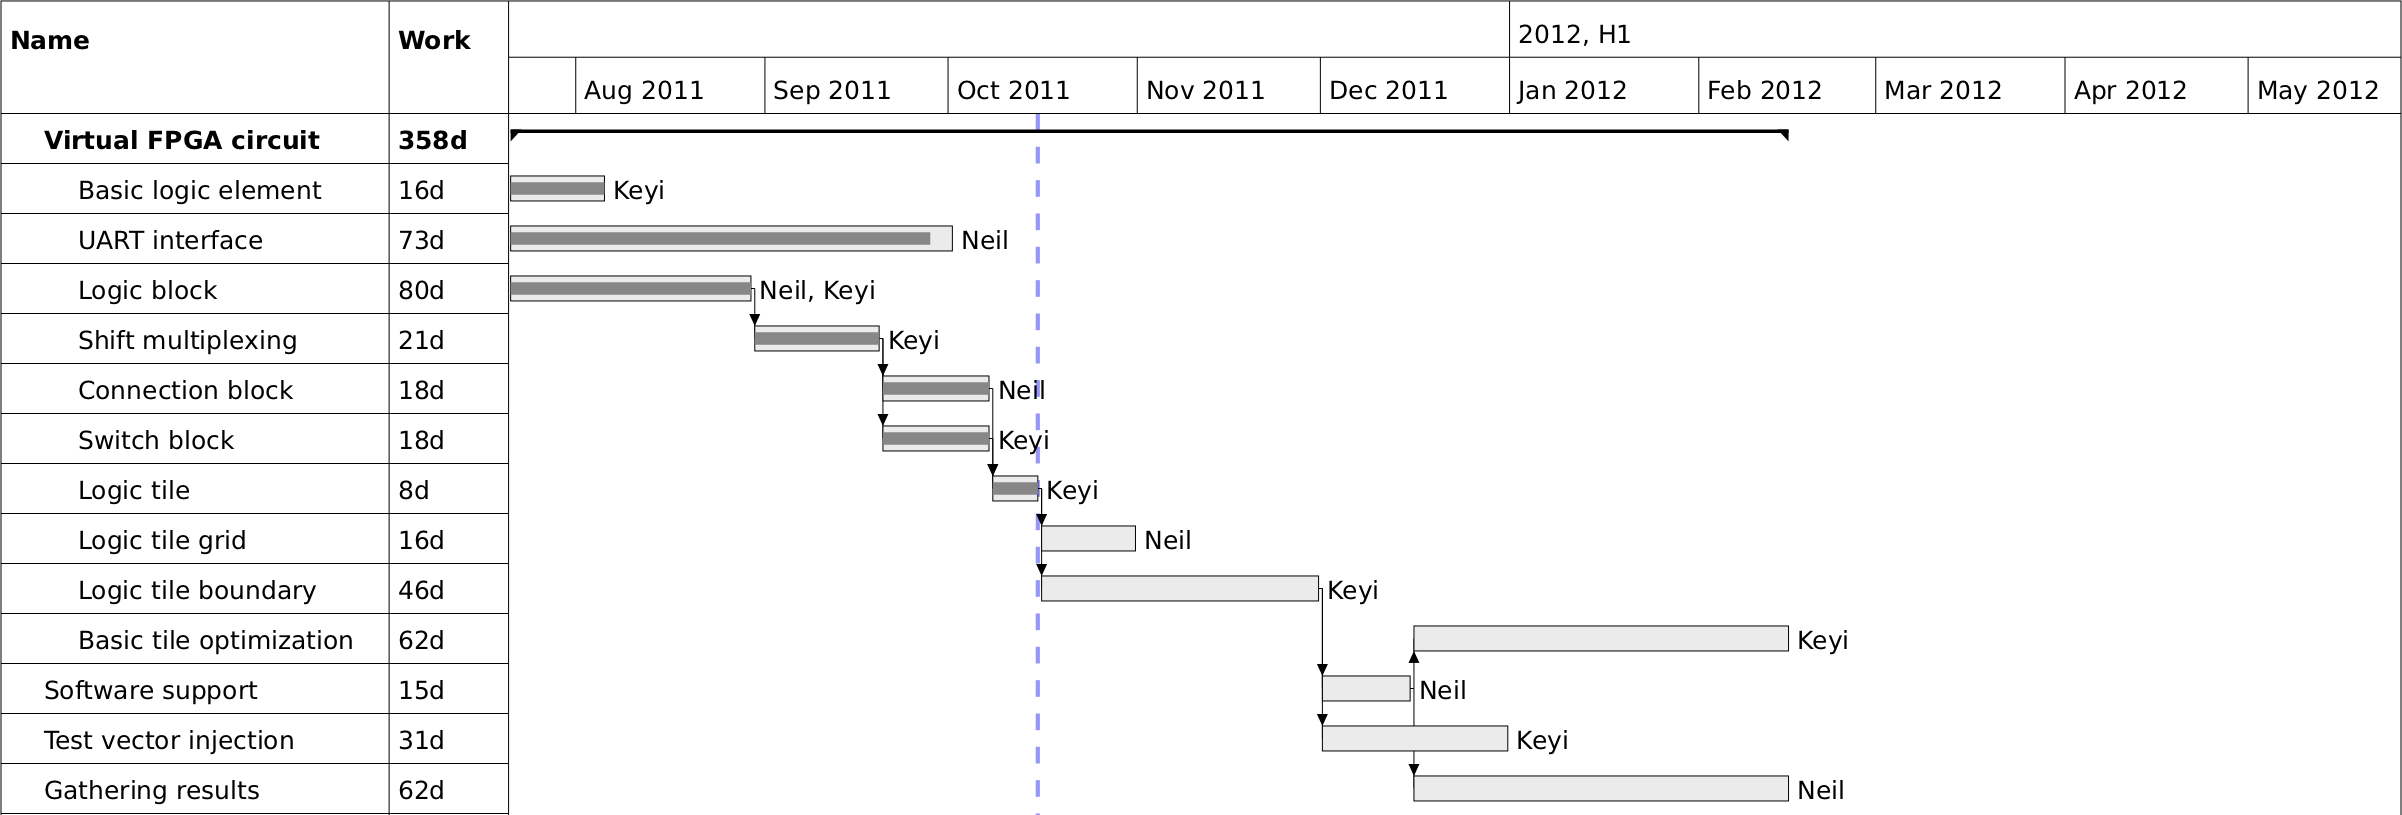
\includegraphics[scale=0.45,angle=90]{gantt.png}


\pagebreak
\section{Test Verilog file}

\begin{tabular}{|p{6.4in}|}
\hline
\begin{verbatim}
 module test(
     clk,
     a, b, c,
     x, y, z
 );

     input clk;
     input a, b, c;
     output x, y, z;

     assign x = a & b;
     assign y = a | b;

     always @ (posedge clk)
         z <= c;

 endmodule
\end{verbatim}
\\ \hline
\end{tabular}

This circuit has 3 outputs, \emph{x}, \emph{y} and \emph{z}.
It contains an AND gate, an OR gate, and a flopped path.
The AND and OR gates allow me to test the tool flow and my bitstream generation software for logic functions that are mostly 0s (AND) and mostly 1s (OR), which is important in the BLIF format, as they are represented in the form that reduces the amount of function lines in the BLIF file.
The flopped path lets me test the way I need to handle internal signals (before and after the flop) and how latches are represented in the BLIF and netlist files.

The result of running placement and routing in \emph{VPR} for a the circuit derived from this verilog is shown in Appendix C.


\pagebreak
\section{VPR Placement and Routing Result}

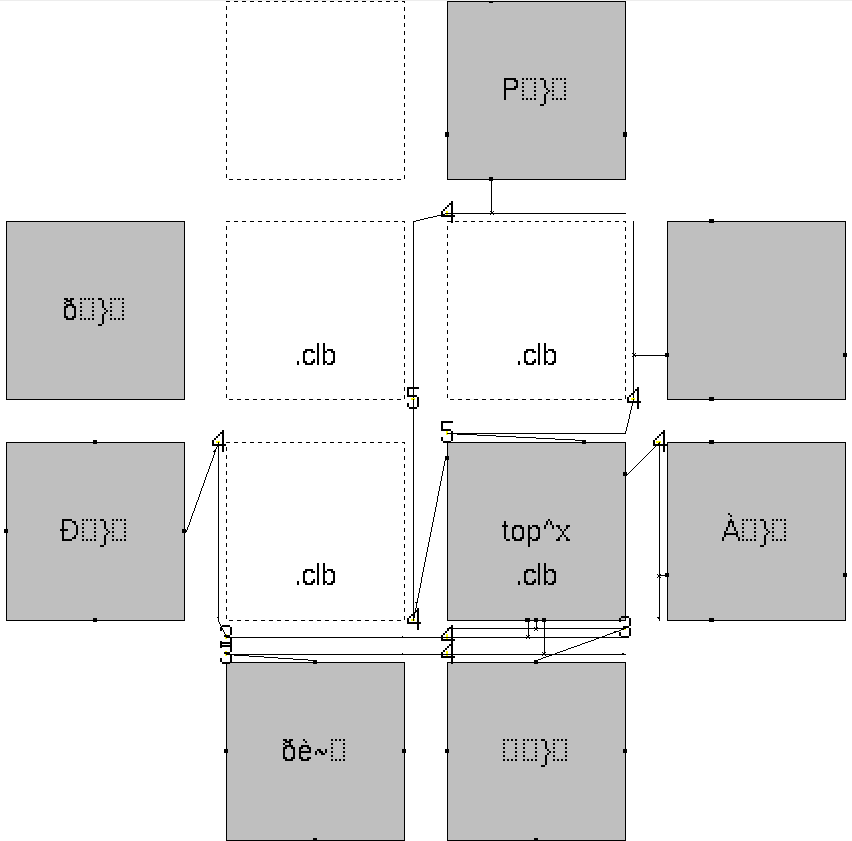
\includegraphics[scale=0.5]{vpr.png}

This is a screenshot from the VPR tool after placement and routing were completed for the test circuit shown in Appendix B.
Placed blocks are shown with a dark grey background and routing tracks are shown as black lines.

Note that there is a VPR issue in rendering the fonts for the IO pad labels.




\end{appendices}

\end{document}


